\documentclass{fenicscourse}

\begin{document}

\fenicslectureoverview{Marie E. Rognes}{NGCM Summer Academy, Southampton, June 23-24 2016}

\begin{frame}
  \frametitle{Course outline}

  %
  % Thursday June 23 2016
  %
  % 1000-1100 (1h)   Overview and installation
  % 1130-1300 (1.5h) L02 Static linear PDEs (Lecture + Hands on)
  % 1430-1600 (1.5h) L03 Static nonlinear PDEs (Lecture + Hands on)
  % 1630-1830 (1.5h) L04 Time-dependent PDEs (Lecture + Hands on)
  %
  %
  % Friday June 24 2016
  %
  % 1000-1100 (1h)   L09 Incompressible Navier-Stokes (Lecture + Hands on)
  % 1130-1300 (1.5h) L13 Introduction to dolfin-adjoint (Lecture)
  % 1430-1600 (1.5h) L16 Optimal control (Lecture + Hands on)
  %

  \begin{itemize}
  \item
    Thursday June 23
    \begin{enumerate}
    \item[L00]
      Introduction to FEniCS and installation
    \item[L02]
      Static linear PDEs
    \item[L03]
      Static nonlinear PDEs
    \item[L04]
      Time-dependent PDEs
    \end{enumerate}

  \item
    Friday June 24
    \begin{enumerate}
    \item[L09]
      Incompressible Navier--Stokes
    \item[L13]
      Introduction to dolfin-adjoint
    \item[L16]
      Optimal control of the Navier-Stokes equations
    \end{enumerate}

  \end{itemize}

  \normalsize

  \bigskip

  \begin{block}{Note}
    Lecture slides and other material (data, input meshes) can also be
    found in the 2016 FEniCS NGCM Training Kit!
  \end{block}

\end{frame}

% The quickest FEniCS intro
\begin{frame}
\medskip

\includegraphics[width=0.99\textwidth]{png/fenics_banner.png}
\begin{columns}[c]
\begin{column}{0.4\textwidth}
\bf{The FEniCS Project is a collection of open-source software
  components aimed at the numerical solution of partial differential
  equations using finite element methods}
\end{column}
\begin{column}{0.7\textwidth}
  \begin{block}{Key distinguishing features}
  \begin{itemize}
  \item
    FEniCS (Python/C++) code is quick to write and easy to read
  \item
    `Any' finite element formulation of 'any' partial differential
    equation can be coded
  \item
    Automated code generation is heavily used under the hood to
    create efficient, specialized, low-level code
  \item
    Performance -- implicit problems with over $12\, 000\, 000\, 000$
    degrees of freedom can be solved in a couple of minutes
  \end{itemize}
  \end{block}
\end{column}
\end{columns}
  \begin{center}
    \colemph{\url{http://fenicsproject.org/}}
  \end{center}
\end{frame}

\begin{frame}
\frametitle{FEniCS has been used for a wide range of
  equations and applications}

{\tiny Reaction-diffusion equations; Stokes with or without nonlinear
  viscosity; compressible and incompressible Navier--Stokes; RANS
  turbulence models; shallow water equations; Bidomain equations;
  nonlinear and linear elasticity; nonlinear and linear
  viscoelasticity; Schr\"odinger; Biot's equations for porous media,
  fracture mechanics, electromagnetism, liquid crystals including
  liquid crystal elastomers, combustion, ... and coupled systems of
  the above, ...}

\begin{center}
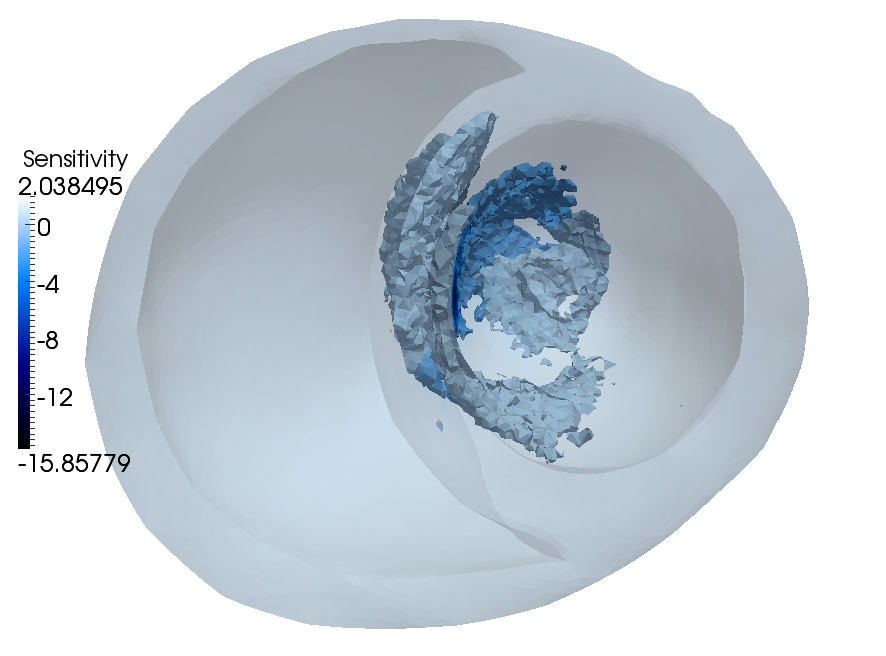
\includegraphics[width=0.24\textwidth]{png/g_el_plusx.png}
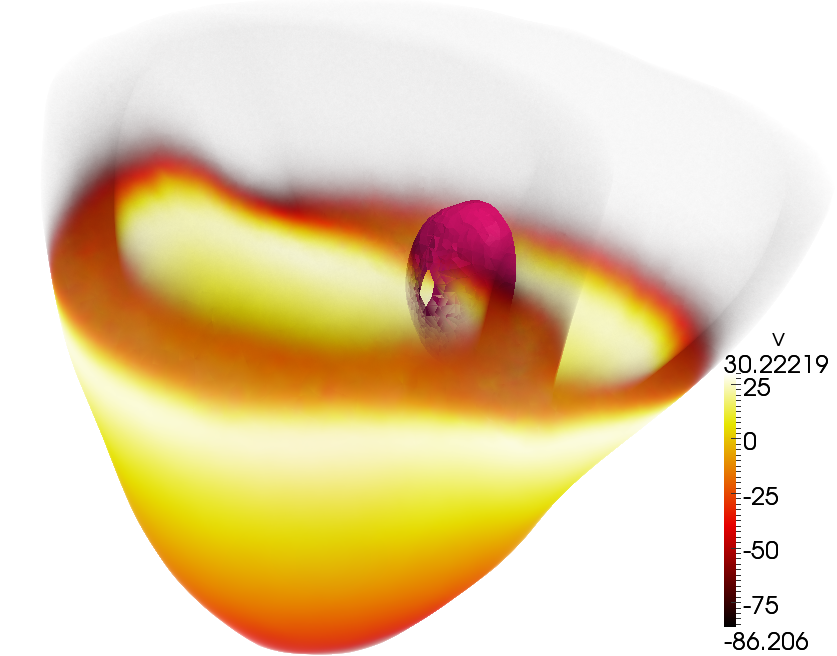
\includegraphics[width=0.24\textwidth]{png/unhealthy_v_at_T200.png}
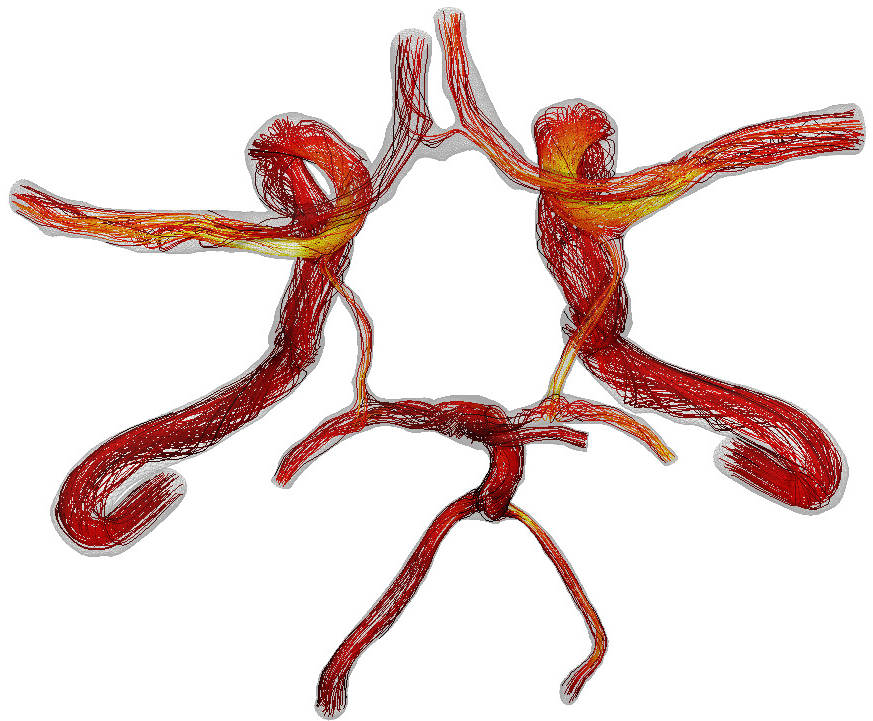
\includegraphics[width=0.24\textwidth]{png/circle_of_willis_simulation.png}
\end{center}

{\tiny for simulating blood flow, computing calcium release in cardic
  tissue, computing the cardiac potential in the heart, simulating
  mantle convection, simulating melting ice sheets, computing the
  optimal placement of tidal turbines, simulating and reconstructing
  tsunamis, simulating the flow of cerebrospinal fluid and the
  deformation of the spinal cord, simulating waveguides, ... }

\end{frame}


% Show a simple taster
\begin{frame}
  \frametitle{Hello World in FEniCS: problem formulation}

  \begin{block}{Poisson's equation}
    \vspace{-0.5cm}
    \begin{displaymath}
      \begin{split}
        -\Delta u &= f \quad \mbox{ in } \Omega \\
        u &= 0 \quad \mbox { on } \partial\Omega
      \end{split}
    \end{displaymath}
  \end{block}

  \begin{block}{Finite element formulation}
    \vspace{1ex}
    Find $u \in V$ such that
    \begin{displaymath}
      \underbrace{\int_{\Omega} \nabla u \cdot \nabla v \dx}_{\textcolor{fenicsred}{a(u,v)}}
      = \underbrace{\int_{\Omega} f \, v \dx}_{\textcolor{fenicsred}{L(v)}}
      \quad \foralls v \in V
    \end{displaymath}
  \end{block}

\end{frame}

\begin{frame}[fragile]
  \frametitle{Hello World in FEniCS: implementation}

    \begin{python}
from fenics import *

mesh = UnitSquareMesh(32, 32)

V = FunctionSpace(mesh, "Lagrange", 1)
u = TrialFunction(V)
v = TestFunction(V)
f = Expression("x[0]*x[1]", degree=2)

a = dot(grad(u), grad(v))*dx
L = f*v*dx

bc = DirichletBC(V, 0.0, DomainBoundary())

u = Function(V)
solve(a == L, u, bc)
plot(u)
    \end{python}

\end{frame}

\begin{frame}
  \frametitle{Basic API}

  \begin{itemize}
  \item
    \texttt{Mesh},
    \texttt{Vertex},
    \texttt{Edge},
    \texttt{Face},
    \texttt{Facet},
    \texttt{Cell}
  \item
    \texttt{FiniteElement}, \texttt{FunctionSpace}
  \item
    \texttt{TrialFunction},
    \texttt{TestFunction},
    \texttt{Function}
  \item
    \texttt{grad()}, \texttt{curl()}, \texttt{div()}, \ldots
  \item
    \texttt{Matrix}, \texttt{Vector}, \texttt{KrylovSolver}, \texttt{LUSolver}
  \item
    \texttt{assemble()}, \texttt{solve()}, \texttt{plot()}
  \end{itemize}

  \vspace{1cm}

  \begin{itemize}
  \item
    Python interface generated semi-automatically by SWIG
  \item
    C++ and Python interfaces almost identical
  \end{itemize}

\end{frame}


% Learning more than what this course covers
\begin{frame}
    \frametitle{Sounds great, but how do I find my way through the
    jungle?}
    \begin{center}
        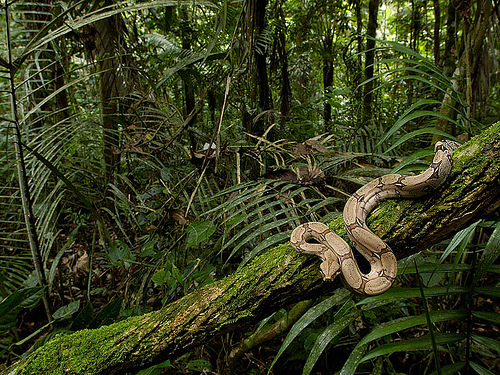
\includegraphics[width=0.8\textwidth]{jpg/jungle10.jpg}
    \end{center}
\end{frame}

\begin{frame}
    \frametitle{Three survival advices}
    \begin{columns}[c]
        \begin{column}{0.33\textwidth}
            \begin{center}
                
\includegraphics[width=0.99\textwidth]{png/python_logo.png}
            \end{center}
        \end{column}
        \begin{column}{0.33\textwidth}
            \begin{center}
                
\includegraphics[width=0.99\textwidth]{jpg/documentation.jpg}\\
            \end{center}
        \end{column}
        \begin{column}{0.33\textwidth}
            \begin{center}
                
\includegraphics[width=0.99\textwidth]{jpg/question-blue.jpg}
            \end{center}
        \end{column}
    \end{columns}
    \begin{columns}[t]
        \begin{column}{0.33\textwidth}
            \begin{center}
                \colemph{Use the right Python tools}
            \end{center}
        \end{column}
        \begin{column}{0.33\textwidth}
            \begin{center}
                \colemph{Explore the documentation}
            \end{center}
        \end{column}
        \begin{column}{0.33\textwidth}
            \begin{center}
                \colemph{Ask, report and request}
            \end{center}
        \end{column}
    \end{columns}
\end{frame}


%% TODO: Update webpage images when readthedocs work is completed

% Demos on old page
\begin{frame}
  \begin{center}
     {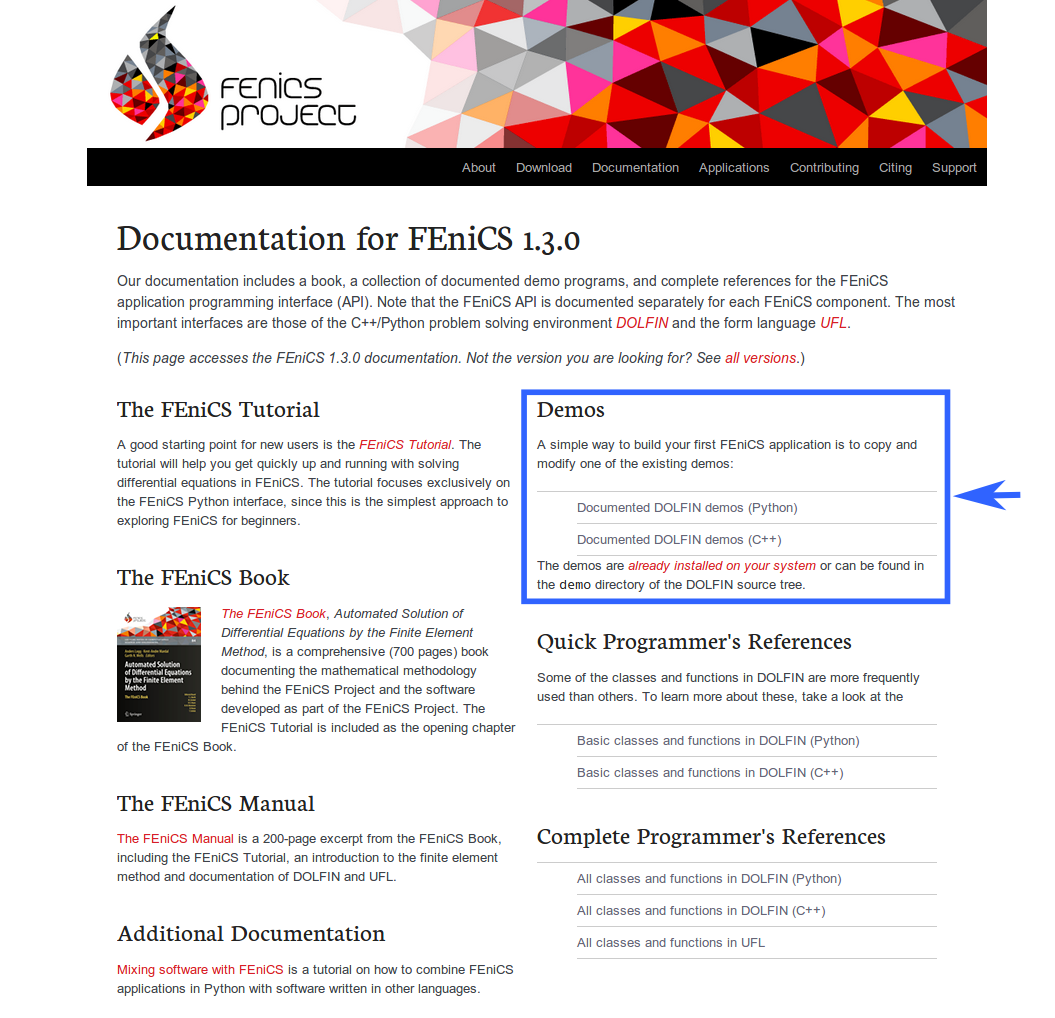
\includegraphics[width=0.80\textwidth]{png/fenics-doc-webpage-5.png}}
    \small
    \colemph{\url{http://fenicsproject.org/documentation/}}
  \end{center}
\end{frame}

% Reference docs on old page
\begin{frame}
  \begin{center}
     {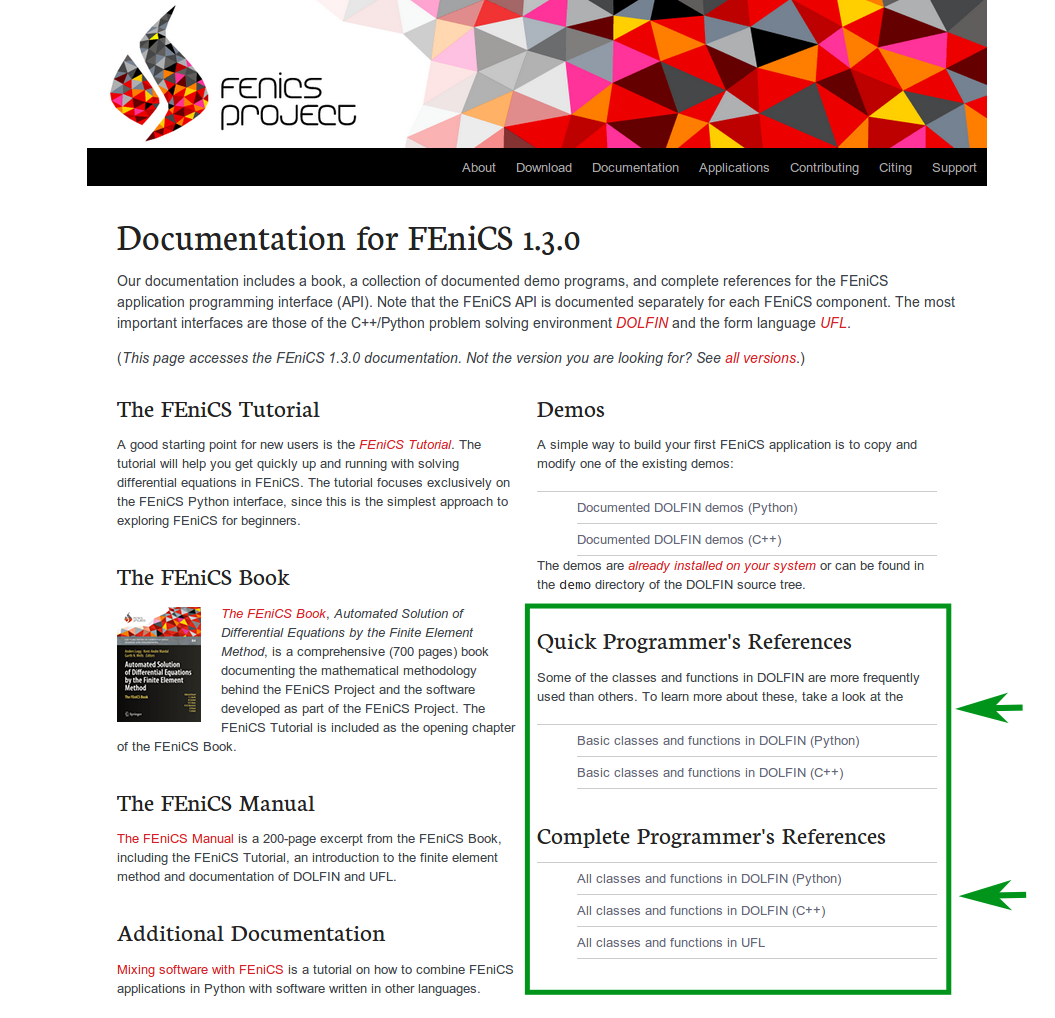
\includegraphics[width=0.80\textwidth]{png/fenics-doc-webpage-6.png}}
    \small
    \colemph{\url{http://fenicsproject.org/documentation/}}
  \end{center}
\end{frame}

% Currently migrating
\begin{frame}
  \begin{center}
     {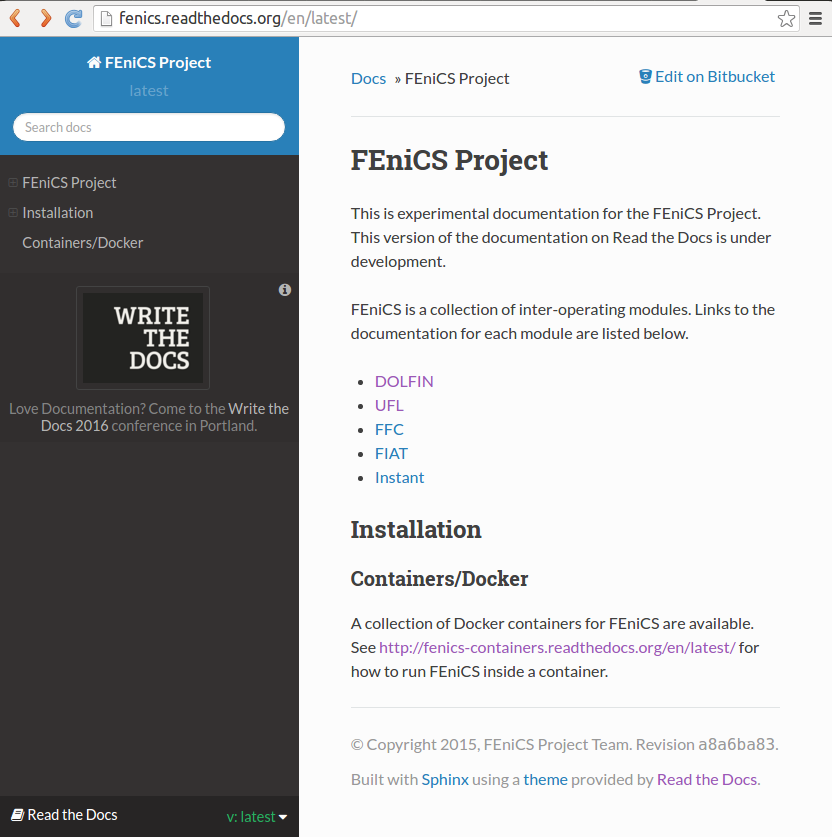
\includegraphics[width=0.80\textwidth]{png/fenics-readthedocs-webpage-1.png}}
    \small
    \colemph{\url{http://fenics.readthedocs.org/}}
  \end{center}
\end{frame}


\begin{frame}
  \frametitle{How to use the FEniCS documentation}

  \alert{\url{http://fenicsproject.org/documentation}}

\end{frame}

\begin{frame}
    \frametitle{Development community is organized via bitbucket.org}
    \begin{center}
        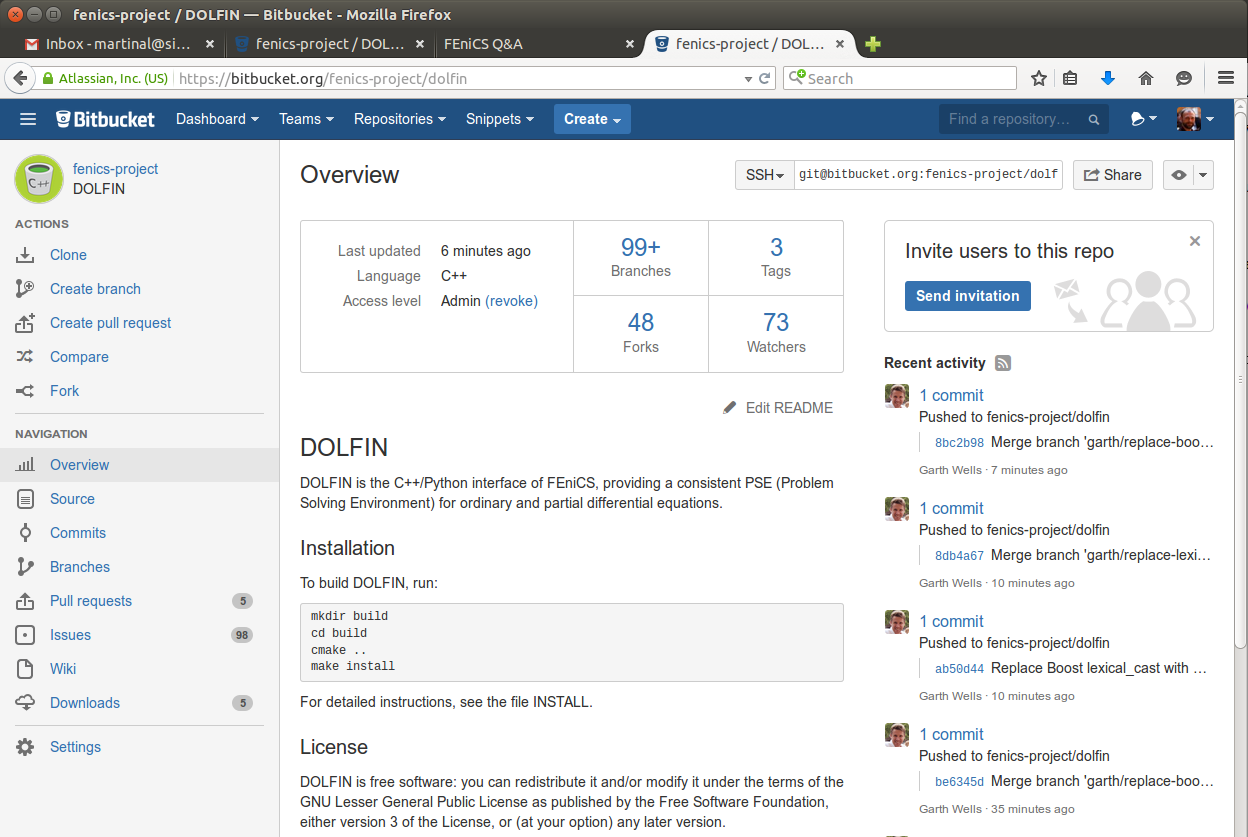
\includegraphics[height=0.75\textheight]{png/fenics-bitbucket-webpage.png}
        \vspace{1em}
        \small
        \colemph{\url{http://bitbucket.org/fenics-project/}}
    \end{center}
\end{frame}
\begin{frame}
    \frametitle{Community help is available via QA forum}
    \begin{center}
        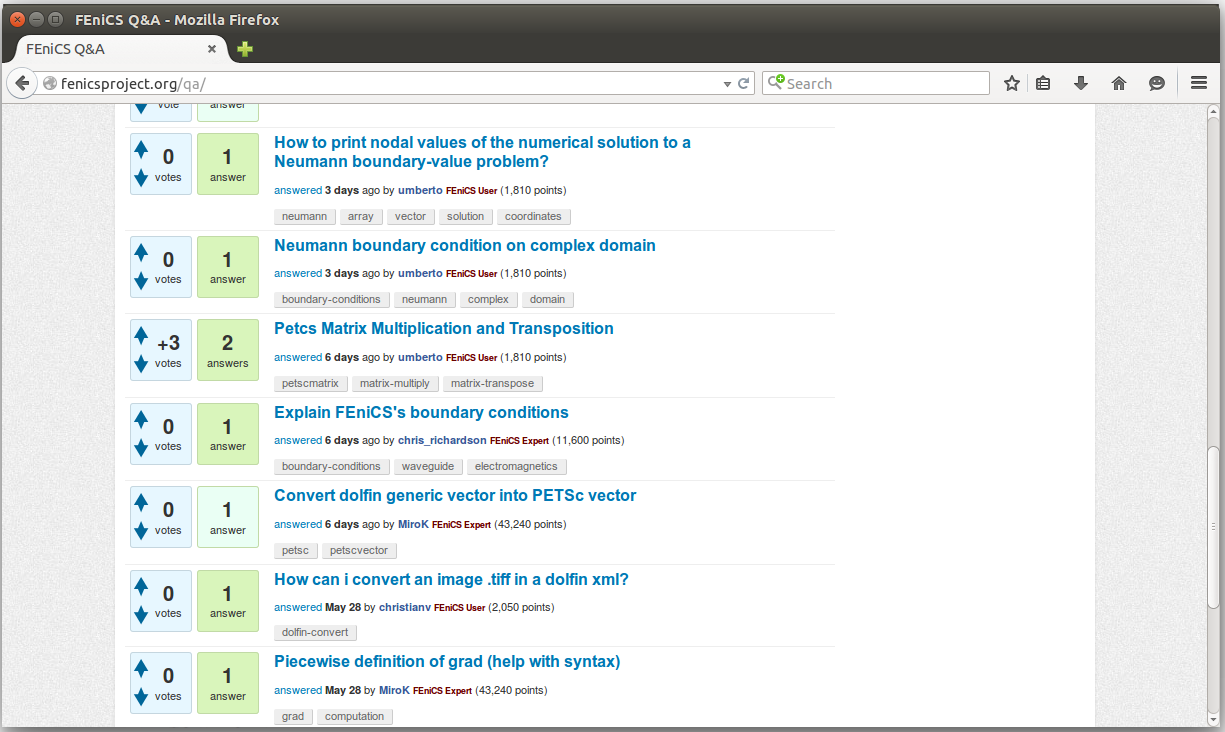
\includegraphics[width=1.0\textwidth,height=0.7\textheight]{png/fenics-qa-website.png}
        \vspace{1em}
        \small
        \colemph{\url{https://fenicsproject.org/qa}}
    \end{center}
\end{frame}


\begin{frame}
  \frametitle{FEniCS Slack Channel}

  \alert{\url{https://fenicsproject.slack.com/}}

\end{frame}

\begin{frame}
  \frametitle{Installation alternatives}

  % FEniCS uses standard setup.py and cmake tools
  % but dependencies are tricky to configure.

  \begin{tabular}{cp{10cm}}
    
\includegraphics[height=1cm]{png/docker_logo.png} &
    \begin{minipage}{10cm}
      \ding{43} Docker images on Linux, Mac, Windows
      \vspace{0.6cm}
    \end{minipage}
    \\
    
\includegraphics[height=1cm]{png/source.png} &
    \begin{minipage}{10cm}
      \ding{43} Build from source with Hashdist (fenics-install.sh)
      \vspace{0.8cm}
    \end{minipage}
    \\
    
\includegraphics[height=1cm]{png/ubuntu_logo.png} &
    \begin{minipage}{10cm}
      \ding{43} PPA with apt packages for Debian and Ubuntu
      \vspace{0.6cm}
    \end{minipage}
    \\
    
\includegraphics[height=1cm]{png/mac_osx_logo.png} &
    \begin{minipage}{10cm}
      \ding{43} Drag and drop installation on Mac OS X
      \vspace{0.8cm}
    \end{minipage}
  \end{tabular}

  \begin{center}
    \colemph{\url{http://fenicsproject.org/download/}}
  \end{center}

\end{frame}


\begin{frame}[fragile]
\frametitle{In this course, follow the instructions from the course web page}

\bigskip

\alert{\url{http://ngcm.soton.ac.uk/summer-academy/fenics.html}}

\bigskip

We'll use (for now)
\begin{itemize}
\item
  Docker
\item
  FEniCS (development version)
\item
  IPython notebook
\end{itemize}


%\begin{center}
%\includegraphics[width=\textwidth]{installation.png}
%\end{center}

\bigskip
Remember that Lectures, code examples and data are provided in your
{\bf FEniCS Training Kits}.

\bigskip

\begin{center}
  \alert{Let's get started!}
\end{center}

\end{frame}


\end{document}
